\section{Construction, Metric, and Resource Effects}
\label{sec:construction-results}

\subsection{RQ3: What Changes Across IBM Constructions and Scale?}

Table~\ref{tab:ibm-baselines} and Fig.~\ref{fig:ibm-baselines} answer the baseline question first. Histogram gradient boosting has the highest mean AUPRC in all eight HI/LI, Small/Medium, early/late contexts. This result is confined to the three recorded baseline families and does not imply that trees dominate AML generally.

\begin{table}[t]
\caption{IBM baseline AUPRC means over ten runs. Bold marks the best of the three recorded families; Fig.~\ref{fig:ibm-baselines} gives uncertainty.}
\label{tab:ibm-baselines}
\centering
\footnotesize
\setlength{\tabcolsep}{2.6pt}
\begin{tabular}{@{}lrrrrr@{}}
\toprule
Cell & HistGB & LR & SAGE & Best & Gap \\
\midrule
HI-SMALL / Early & \textbf{0.0657} & 0.0144 & 0.0038 & HistGB & 0.0514 \\
HI-SMALL / Late & \textbf{0.0964} & 0.0173 & 0.0071 & HistGB & 0.0792 \\
HI-MEDIUM / Early & \textbf{0.0890} & 0.0139 & 0.0248 & HistGB & 0.0641 \\
HI-MEDIUM / Late & \textbf{0.1693} & 0.0157 & 0.0371 & HistGB & 0.1322 \\
LI-SMALL / Early & \textbf{0.0126} & 0.0039 & 0.0021 & HistGB & 0.0087 \\
LI-SMALL / Late & \textbf{0.0171} & 0.0040 & 0.0022 & HistGB & 0.0130 \\
LI-MEDIUM / Early & \textbf{0.0143} & 0.0037 & 0.0069 & HistGB & 0.0073 \\
LI-MEDIUM / Late & \textbf{0.0297} & 0.0040 & 0.0078 & HistGB & 0.0219 \\
\bottomrule
\end{tabular}
\end{table}


\begin{figure}[t]
  \centering
  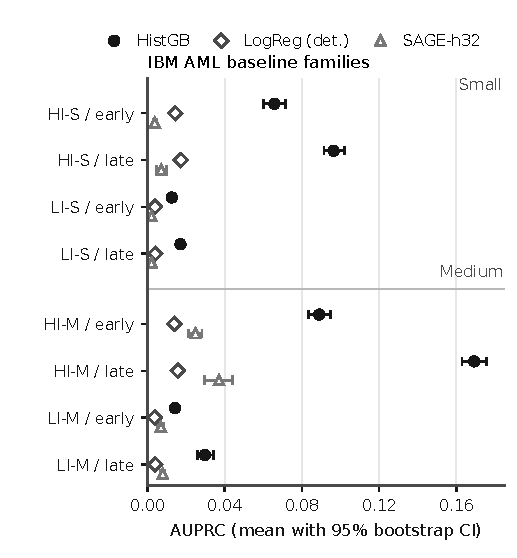
\includegraphics[width=\columnwidth]{figures/fig03_ibm_metric_scale_construction.pdf}
  \caption{IBM baseline-family AUPRC. Points are ten-run means and whiskers are deterministic 95\% bootstrap intervals. Deterministic LR cells retain zero-width intervals.}
  \label{fig:ibm-baselines}
\end{figure}

The graph-construction grid answers a different question. GINE h64 has the highest mean AUPRC in all four feasible Small contexts, whereas Medium GINE has no performance observation. Table~\ref{tab:ibm-construction} identifies the best measured non-reference construction by AUPRC in each cell and reports that same construction's matched changes on all three metrics. It is not a multi-metric winner table.

\begin{table*}[t]
\caption{Best measured non-reference IBM construction by AUPRC in each cell. Deltas compare that same construction with h64 on AUPRC, AUROC, and F1. The Holm value is the dependence-aware size-level AUPRC test over ten seed blocks, not a context-specific test.}
\label{tab:ibm-construction}
\centering
\footnotesize
\setlength{\tabcolsep}{3.0pt}
\begin{tabularx}{\textwidth}{@{}lrrrrrrX@{}}
\toprule
Cell & Ref AUPRC & Best construction & $\Delta$AUPRC & $\Delta$AUROC & $\Delta$F1 & Holm $p$ & Feasibility \\
\midrule
HI-SMALL / Early & 0.0103 & GINE & +0.0158 & +0.0290 & -0.0031 & 0.014 & Small measured \\
HI-SMALL / Late & 0.0110 & GINE & +0.0203 & +0.0354 & -0.0020 & 0.014 & Small measured \\
HI-MEDIUM / Early & 0.0424 & Degree & -0.0172 & -0.1130 & -0.0008 & 0.012 & GINE Medium blocked \\
HI-MEDIUM / Late & 0.0500 & Degree & -0.0174 & -0.1170 & +0.0054 & 0.012 & GINE Medium blocked \\
LI-SMALL / Early & 0.0032 & GINE & +0.0066 & -0.0028 & -0.0012 & 0.014 & Small measured \\
LI-SMALL / Late & 0.0057 & GINE & +0.0049 & -0.0180 & -0.0020 & 0.014 & Small measured \\
LI-MEDIUM / Early & 0.0103 & Recent & -0.0037 & +0.0312 & +0.0007 & 0.012 & GINE Medium blocked \\
LI-MEDIUM / Late & 0.0111 & Degree & -0.0033 & -0.0440 & -0.0025 & 0.012 & GINE Medium blocked \\
\bottomrule
\end{tabularx}
\end{table*}


Matched controls show that transaction attributes carry ranking information for the h64 classifier. Zeroing edge features lowers AUPRC relative to the reference by $0.00267$ on Small (seed-block CI $[-0.00424,-0.00109]$, Holm $p=0.0820$) and $0.01206$ on Medium (CI $[-0.01395,-0.01022]$, Holm $p=0.0117$). The Small corrected test is not significant, although all four context means are negative. Shuffling those features lowers AUPRC by $0.00330$ on Small (Holm $p=0.0137$) and $0.01208$ on Medium ($p=0.0117$); again, all context means are negative. These interventions preserve either the graph or feature marginals, so they support a bounded alignment result for this classifier, strongest on Medium and for the shuffled control. They do not prove that the attributes causally improve every fraud model.

Construction effects also change with scale and metric. Degree capping raises Small mean F1 by $0.00473$ and AUROC by $0.02354$, but none of its Small AUPRC, AUROC, or F1 tests survives Holm correction. On Medium it raises F1 by $0.00587$ (Holm $p=0.0352$) while reducing AUPRC by $0.02086$ ($p=0.0117$). The recent-window graph shows a different Medium tradeoff: AUROC rises by $0.02525$ ($p=0.0117$) and F1 by $0.00419$ ($p=0.0352$), while AUPRC falls by $0.01324$ ($p=0.0117$). Figure~\ref{fig:ablation-effects} places all three matched metric effects on one scale. These are fixed-grid empirical interactions, not identified mechanisms; truncating history changes information, degrees, and computation at once.

\begin{figure*}[t]
  \centering
  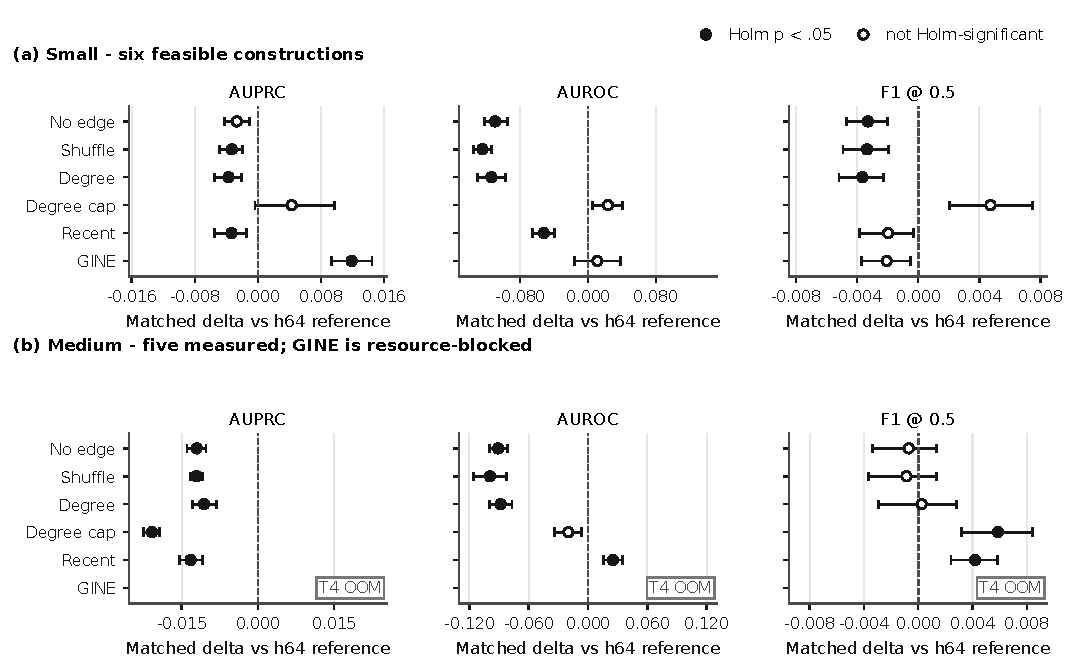
\includegraphics[width=\textwidth]{figures/fig05_matched_ablation_effects.pdf}
  \caption{Candidate-minus-reference IBM effects for AUPRC, AUROC, and F1. The four fixed contexts are averaged within seed before interval estimation and testing ($n=10$ seed blocks). GINE is Small-only; a construction can help one metric while reducing another.}
  \label{fig:ablation-effects}
\end{figure*}

\subsection{RQ4: When Do Ranking and Decision Metrics Disagree?}

AUPRC and F1 select different winners in 11 of 16 feasible variant--protocol contexts: three of eight baseline-grid contexts and all eight graph-grid contexts. This count is specific to the saved F1 threshold of 0.5; it is not a threshold-invariant decision result. Figure~\ref{fig:rank-divergence} shows the clearest example. In HI-Medium late-window evaluation, the h64 reference ranks first of six graph configurations by AUPRC ($0.0500$) but sixth by F1 ($0.0127$). Degree capping ranks sixth by AUPRC ($0.0127$) and first by F1 ($0.0221$). RecentWindow ranks first by AUROC ($0.9333$), fifth by AUPRC, and second by F1.

\begin{figure}[t]
  \centering
  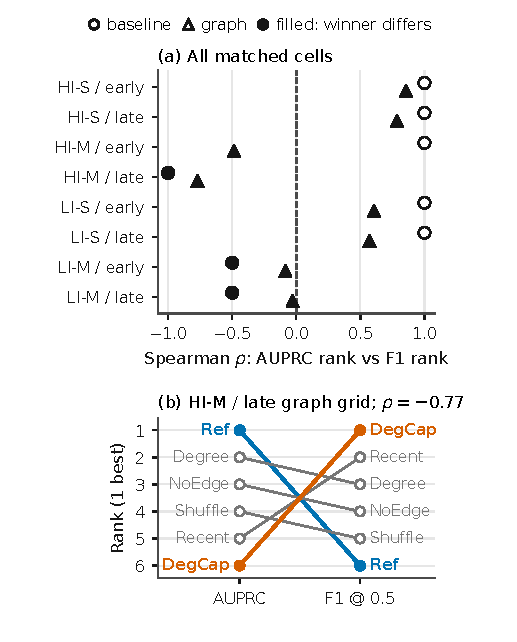
\includegraphics[width=\columnwidth]{figures/fig04_rank_decision_divergence.pdf}
  \caption{AUPRC--F1 rank association and the HI-Medium late-window reversal. F1 uses the saved 0.5 threshold; AUPRC integrates score ordering.}
  \label{fig:rank-divergence}
\end{figure}

The GINE result makes the distinction concrete. Against the h64 reference on the four Small contexts, GINE raises mean AUPRC by $0.01190$ (seed-block CI $[0.00934,0.01447]$, $d_z=2.70$, Holm $p=0.0137$); every context mean is positive. Its mean F1 is lower by $0.00206$ (CI $[-0.00371,-0.00052]$), but that dependence-aware corrected test is not significant ($p=0.252$). A high AUROC can likewise coexist with modest precision in a rare-positive task. Monotone recalibration may change fixed-threshold decisions, but it preserves score order and therefore cannot repair an AUPRC or AUROC ranking \cite{guo2017calibration,saerens2002prior}.

\subsection{RQ5: What Does the Resource Contract Exclude?}

Resource cost changes the admissible comparison set. Averaged over the four Small contexts, GINE takes $449.47$ seconds versus $49.31$ seconds for the h64 reference, about nine times longer. On Medium, RecentWindow averages $141.65$ seconds versus $275.19$ seconds for the reference, while exchanging lower AUPRC for higher AUROC and F1. Figure~\ref{fig:runtime-pareto} marks Pareto status only within a common variant and protocol; it does not merge runtimes from different tasks or hardware records. Table~\ref{tab:resource-boundaries} states how the unmeasured cells enter the benchmark.

\begin{figure*}[t]
  \centering
  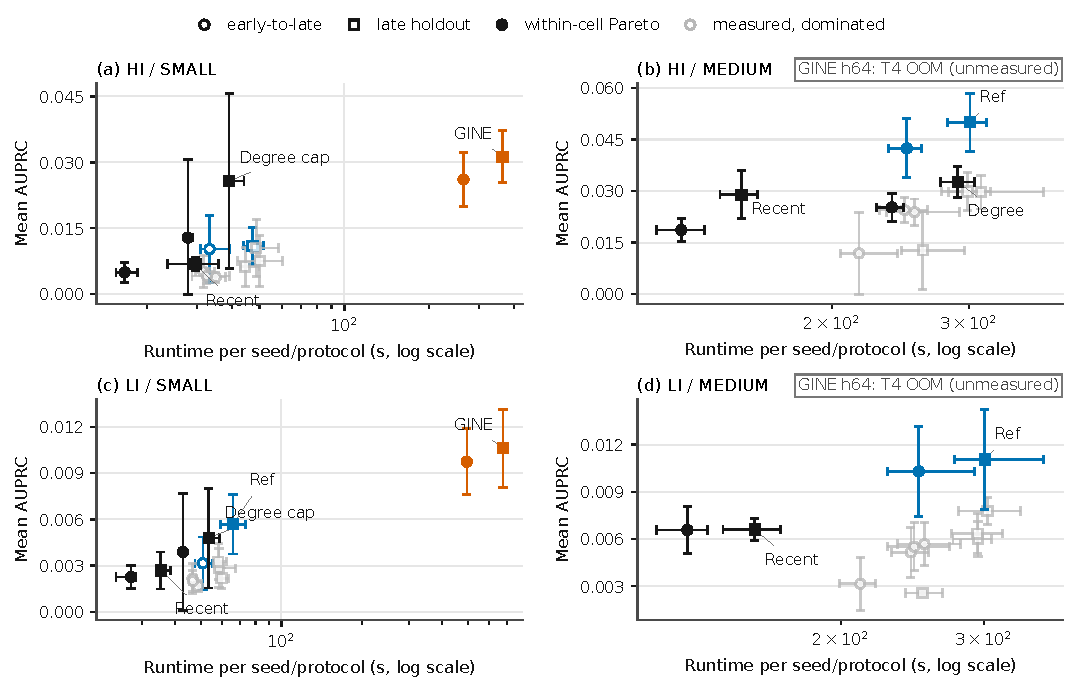
\includegraphics[width=\textwidth]{figures/fig06_runtime_resource_pareto.pdf}
  \caption{Configuration-specific AUPRC and elapsed time under the recorded IBM envelope. Pareto status is computed only within a variant--protocol cell. Medium GINE and both Large variants remain nonnumeric and outside predictive ordering.}
  \label{fig:runtime-pareto}
\end{figure*}

\begin{table}[t]
\caption{Unmeasured resource cells. Status is a feasibility outcome under the declared envelope, never a predictive score.}
\label{tab:resource-boundaries}
\centering
\footnotesize
\setlength{\tabcolsep}{2.2pt}
\begin{tabularx}{\columnwidth}{@{}p{0.23\columnwidth}p{0.18\columnwidth}p{0.24\columnwidth}X@{}}
\toprule
Cell & Envelope & Status & Benchmark treatment \\
\midrule
IBM AML HI-Large & safe resource guard & \textsc{guard-\allowbreak blocked} & excluded from predictive ranks, matched means, and Pareto sets \\
IBM AML LI-Large & safe resource guard & \textsc{guard-\allowbreak blocked} & excluded from predictive ranks, matched means, and Pareto sets \\
IBM AML HI-Medium GINE h64 & single Tesla T4 CUDA OOM & \textsc{t4-oom} & excluded from predictive ranks, matched means, and Pareto sets \\
IBM AML LI-Medium GINE h64 & single Tesla T4 CUDA OOM & \textsc{t4-oom} & excluded from predictive ranks, matched means, and Pareto sets \\
DGraphFin GAT h64/l2 & Tesla T4 CUDA OOM & \textsc{t4-oom} & excluded from predictive ranks, matched means, and Pareto sets \\
DGraphFin GraphSAGE max-pool rerun & larger GPU required & \textsc{unmeasured} & excluded from predictive ranks, matched means, and Pareto sets \\
\bottomrule
\end{tabularx}
\end{table}


The two Medium GINE lanes each exhausted Tesla T4 memory before producing any of 20 planned outputs. HI-Large and LI-Large were stopped by the safe resource guard and likewise have zero results and predictions. The fixed DGraphFin GAT h64/l2 cell is also T4-OOM; an h32/l1 diagnostic cannot fill that cell because it changes the model. These statuses answer feasibility questions under recorded envelopes. They say nothing about predictive performance on larger hardware.
